% RAGFailBench, IEEE BigData 2026 camera-ready.
% Build: tectonic paper/main.tex   (or pdflatex main && pdflatex main)
% Numbers come from reports/pilot_stability/paper/ (tables*.md) and
% reports/regression/; see reports/pilot_stability/paper/revision_text.md.
\documentclass[conference]{IEEEtran}
\IEEEoverridecommandlockouts
\usepackage{cite}
\usepackage{amsmath,amssymb}
\usepackage{graphicx}
\usepackage{booktabs}
\usepackage{multirow}
\usepackage{array}
\usepackage{tikz}
\usetikzlibrary{arrows.meta,positioning,fit,calc}
\usepackage[hidelinks]{hyperref}
\usepackage{xcolor}

\newcommand{\op}[1]{\texttt{\detokenize{#1}}}
\newcommand{\pp}{\,pp}
\renewcommand{\arraystretch}{1.08}
\setlength{\tabcolsep}{3.6pt}
\setlength{\emergencystretch}{1.5em}

\begin{document}

\title{RAGFailBench: Automated Construction and Controllable Failure-Injection Benchmarking for Retrieval-Augmented Generation}

\author{\IEEEauthorblockN{Taixing Bi}
\IEEEauthorblockA{Independent Researcher\\
New York, NY, USA\\
taixingbijob@gmail.com}}

\maketitle

\begin{abstract}
Most RAG benchmarks are released once and go stale as the underlying knowledge base changes.
RAGFailBench instead regenerates a failure-aware benchmark whenever the corpus changes. It
builds provenance-preserving question-answering (QA) seeds from a document corpus, validates
them with rule checks, an LLM judge and a baseline-model test, audits a sample by hand, and
injects six parameterized failure operators under a fixed eight-passage context budget. Each
failure case is compared with its own parent clean seed, so a drop is attributable to one
operator. On a 768-page Wikipedia pilot (12,366 chunks), three seeded runs give a stable
construction funnel (QA acceptance 74.8\%\,$\pm$\,1.0\%; failure verification 94.9\%\,$\pm$\,0.3\%).
A blind human audit accepts 84.0\% of sampled seeds (95\% CI 71.5--91.7\%) and judges 96.3\% of
sampled failure cases valid. Evaluating three Bedrock-hosted models shows that conflicting
evidence is the dominant failure for all of them (26.6--30.4-point paired drop), that they
abstain correctly on 92--98\% of evidence-absent cases, and that context noise and evidence
position cause no measurable drop with eight passages. On two Wikipedia snapshots three months
apart, the regression gate passes the corpus update and blocks a retrieval-depth change
(top-$k$ 8$\to$4) that leaves clean accuracy unchanged. Code, configurations and all run
artifacts are released.
\end{abstract}

\begin{IEEEkeywords}
retrieval-augmented generation, benchmark construction, regression testing, failure injection, LLM evaluation, reproducibility
\end{IEEEkeywords}

\section{Introduction}
Knowledge bases behind retrieval-augmented generation (RAG) systems change continuously: pages
are edited, reorganized and retired, and every change is followed by re-indexing and
redeployment. In practice such deployments are often checked against a small, manually written
``golden'' QA set that is rarely revisited. That set says little about the failure modes a RAG
system meets in production: evidence that has been deleted, passages that look relevant but do
not contain the answer, answers split across chunk boundaries, and documents that contradict
each other after a partial update.

Existing RAG benchmarks do not close this gap. The modeling paradigm is well established
\cite{lewis2020rag,gao2023survey,zhao2024survey,huang2024survey}, but benchmarks and evaluation
frameworks such as RAGAS, ARES, RGB, RAGBench and CRUD-RAG score systems against data fixed at
release time \cite{es2024ragas,saadfalcon2024ares,chen2024rgb,friel2024ragbench,lyu2024crud}.
Tools that generate test sets from a user corpus, such as the RAGAS test-set generator and
YourBench \cite{es2024ragas,shashidhar2025yourbench}, produce clean questions but no typed,
controllable failure conditions. Teams therefore cannot answer a recurring question: after this
week's document changes, did robustness regress, and against which failure mode?

RAGFailBench addresses this with (i) automatic construction of validated,
provenance-preserving QA seeds from a corpus snapshot and (ii) six typed, parameterized failure
operators that turn each seed into labeled failure cases. Models are evaluated on clean and
failure conditions under the same context budget, and each failure case is compared with its
own parent seed.

\subsection{Contributions}
\textbf{C1, automated construction.} A configuration-driven pipeline that ingests a corpus,
generates QA pairs with supporting-sentence provenance, filters them with documented rule,
judge and baseline checks, and audits a stratified sample by hand.

\textbf{C2, controlled failure injection.} Six operators anchored to the RAG pipeline stage they
corrupt, each with three severities, a fixed eight-passage budget, automatic leak checks and an
independent LLM audit of every abstain-expected case.

\textbf{C3, regression workflow, tested.} The benchmark is regenerated from a new corpus
snapshot and compared with a gate that reports a per-operator decision with bootstrap CIs. We
run it on two Wikipedia snapshots and on a deliberately degraded retrieval configuration.

We ask \textbf{RQ1}: how much does each operator cost, measured against matched parents?
\textbf{RQ2}: do models differ in sensitivity to specific operators? \textbf{RQ3}: does a
regenerated benchmark catch a regression that clean accuracy misses?

\section{Related Work}
\textbf{RAG and its evaluation.} Lewis et al.\ introduced RAG \cite{lewis2020rag}; in-context
retrieval augmentation works without changing the model \cite{ram2023incontext}; surveys chart
its architectures \cite{gao2023survey,zhao2024survey,huang2024survey}. RAGAS computes
reference-free faithfulness and relevance scores \cite{es2024ragas}, ARES trains lightweight
judges on synthetic data \cite{saadfalcon2024ares}, RGB probes noise robustness, negative
rejection and counterfactual robustness \cite{chen2024rgb}, and RAGBench and CRUD-RAG extend
domain and update coverage \cite{friel2024ragbench,lyu2024crud}. All evaluate against a fixed
dataset. RAGFailBench treats the dataset itself as regenerable and every stress condition as a
typed operator with a matched clean parent.

\textbf{Stressors studied in isolation.} Each operator re-implements, inside one regenerable
pipeline, a stressor with its own literature. Position effects in long contexts were shown by
Liu et al.\ \cite{liu2024lost} (\op{evidence_position}); the effect of irrelevant and related
passages on RAG by Cuconasu et al.\ \cite{cuconasu2024noise} (\op{context_noise},
\op{hard_negative}); and conflicts between retrieved evidence and parametric knowledge by
Longpre et al.\ \cite{longpre2021entity} and ClashEval \cite{wu2024clasheval}
(\op{conflict}). Our contribution is not a new stressor but the construction, validation and
regeneration around them.

\textbf{QA construction and retrieval.} SQuAD, Natural Questions, TriviaQA, HotpotQA and KILT
established the formats most RAG evaluation still uses
\cite{rajpurkar2016squad,kwiatkowski2019nq,joshi2017triviaqa,yang2018hotpotqa,petroni2021kilt}
but were built once by large annotation efforts. RAGFailBench automates supporting-sentence QA
construction so it can be rerun on a new snapshot. Sparse and dense retrievers
\cite{robertson2009bm25,karpukhin2020dpr,izacard2022contriever,khattab2020colbert,santhanam2022colbertv2}
and BEIR \cite{thakur2021beir} evaluate retrieval itself; RAGFailBench does not run a retriever
and does not measure Recall@$k$, MRR or nDCG (Section~\ref{sec:scope}).

\textbf{LLM judges and tooling.} We use an LLM correctness judge in the spirit of G-Eval
\cite{liu2023geval}, and validate it against human labels. Industry tools such as LangSmith,
OpenAI Evals, DeepEval and Promptfoo \cite{langsmith,openaievals,deepeval,promptfoo} execute
test sets but assume the set already exists; holistic benchmarks such as HELM and MTEB
\cite{liang2022helm,muennighoff2023mteb} motivate per-condition rather than single-score
reporting. Our regeneration loop follows continuous-integration and regression-test-selection
practice \cite{fowler2006ci,rothermel1996regression}.

\begin{table}[t]
\centering
\caption{Capability comparison with prior RAG evaluation systems.}
\label{tab:compare}
\footnotesize
\resizebox{\columnwidth}{!}{%
\begin{tabular}{@{}lcccc@{}}
\toprule
System & Auto.\ constr. & Typed failures & Regenerable & Regr.\ gate \\
\midrule
RAGAS \cite{es2024ragas} & partial & -- & -- & metrics only \\
ARES \cite{saadfalcon2024ares} & synthetic & -- & -- & metrics only \\
RGB \cite{chen2024rgb} & partial & partial & -- & -- \\
RAGBench \cite{friel2024ragbench} & \checkmark & -- & -- & -- \\
CRUD-RAG \cite{lyu2024crud} & \checkmark & partial & -- & -- \\
YourBench \cite{shashidhar2025yourbench} & \checkmark & -- & \checkmark & -- \\
RAGFailBench & \checkmark & \checkmark\ (6) & \checkmark & \checkmark \\
\bottomrule
\end{tabular}}
\end{table}

\section{Framework}
\label{sec:framework}
RAGFailBench is a linear pipeline (Fig.~\ref{fig:loop}): a corpus snapshot is filtered and
chunked; candidate QA pairs are generated and validated automatically; a sample of the
accepted seeds is audited by hand; seeds are turned into failure cases; and clean and failure
cases are evaluated and compared with a previous run.

\begin{figure*}[t]
\centering
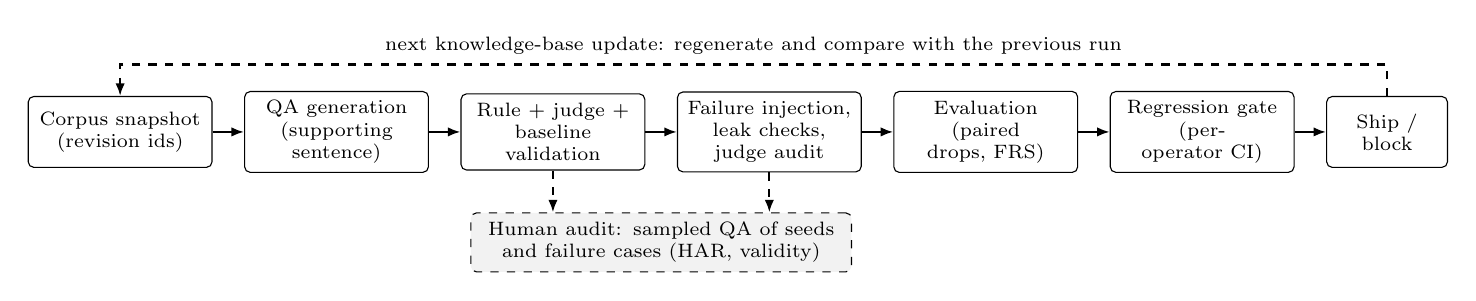
\begin{tikzpicture}[
  node distance=4mm,
  box/.style={draw, rounded corners=2pt, align=center, font=\scriptsize, minimum height=9mm, text width=21mm, fill=white},
  hum/.style={box, dashed, fill=gray!10},
  arr/.style={-{Latex[length=1.6mm]}, thick}]
\node[box] (corpus) {Corpus snapshot\\(revision ids)};
\node[box, right=of corpus] (gen) {QA generation\\(supporting sentence)};
\node[box, right=of gen] (val) {Rule + judge +\\baseline validation};
\node[box, right=of val] (inj) {Failure injection,\\leak checks, judge audit};
\node[box, right=of inj] (eval) {Evaluation\\(paired drops, FRS)};
\node[box, right=of eval] (gate) {Regression gate\\(per-operator CI)};
\node[box, right=of gate, text width=13mm] (dec) {Ship /\\block};
\node[hum, text width=46mm, minimum height=7mm] (audit) at ($(val.south)!0.5!(inj.south)+(0,-9mm)$) {Human audit: sampled QA of seeds and failure cases (HAR, validity)};
\foreach \a/\b in {corpus/gen, gen/val, val/inj, inj/eval, eval/gate, gate/dec} \draw[arr] (\a) -- (\b);
\draw[arr, dashed] (val.south) -- (val.south |- audit.north);
\draw[arr, dashed] (inj.south) -- (inj.south |- audit.north);
\draw[arr, dashed] (dec.north) -- ++(0,4mm) -| node[pos=0.25, above, font=\scriptsize] {next knowledge-base update: regenerate and compare with the previous run} (corpus.north);
\end{tikzpicture}
\caption{The RAGFailBench loop. A knowledge-base update triggers re-ingestion, automatic regeneration of seeds and
failure cases, evaluation, and a gated decision. The human audit (dashed) is sampled quality assurance of accepted
seeds and failure cases; it reports HAR and failure validity and does not approve every item.}
\label{fig:loop}
\end{figure*}

\subsection{Corpus}
The pilot corpus is fetched through the MediaWiki API \cite{mediawiki}: 1,000 English
Wikipedia pages \cite{wikipedia} (200 per category: person, location, science/technology,
historical event, organization/product). Disambiguation and stub pages are removed and pages
are deduplicated, leaving 768 pages, which section-aware chunking splits into 12,366 chunks.
Every page's revision id is recorded, so a snapshot can be re-fetched exactly. The source module
is a pluggable adapter; only Wikipedia is evaluated here.

\subsection{QA generation}
Candidate QA pairs are generated per chunk by Qwen3-32B (Table~\ref{tab:config}), which returns a
question, an answer and the supporting sentence that justifies it. The prompt names the source
article and requires the question to name its subject (``When did Albert Einstein die?'', not
``When did he die?''). Retaining the supporting sentence is what lets the absence operators
remove exactly the justifying evidence. Generation follows a difficulty quota (40\% easy,
40\% medium, 20\% hard).

\subsection{Automatic validation}
\label{sec:validation}
Candidates first pass deterministic rule checks on normalized text: \emph{uniqueness}
(a who/which/what question with a person or organization answer whose supporting sentence lists
other entities joined by ``and''), \emph{containment} (the gold answer occurs in the supporting
sentence, which occurs in the chunk), \emph{refers-to-passage} (``the passage'',
``mentioned''), \emph{time-sensitive phrasing} (``current'', ``latest'', an undated ``as of''),
\emph{answer in question}, \emph{unresolved referent} (a pronoun with no name before it, or a
possessive or ``the company''-style phrase in a question that names nothing),
\emph{title-only} (a question that only asks what the page title is), \emph{multi-part}
(``when and where'', ``\dots, and what'') and length limits. Rule-passing candidates are then
assessed in parallel by an LLM answerability judge (answerable, supported, unique, clear, with a
confidence) and a baseline test in which a reference model answers from the gold chunk alone.
Accepted candidates are deduplicated (exact or character-5-gram Jaccard $\ge$\,0.85) and a
stratified sample of 200 per run becomes the clean seeds.

The quality score $q = 0.3\,[\text{rules}] + 0.1\,[\text{unique}] + 0.3\,c\,(a{+}s{+}u{+}k)/4 +
0.3\max(F_1^{\text{base}}, [\text{base correct}])$ combines these signals ($a,s,u,k$ are the
judge's verdicts and $c$ its confidence). A threshold sweep shows that $q$ never makes a
decision on its own: every candidate passing the hard gates scores $\ge$\,0.985, and a rule
failure caps $q$ at 0.70, so any threshold from 0 to 0.95 accepts the same candidates. We report
$q$ as a ranking score, not a filter. The multi-part rule was added after the runs and applied to
the selected seeds, removing 11, 16 and 12 of 200 (with all their failure cases and evaluation
rows); every drop is paired by parent, so removing a parent keeps comparisons matched.

\subsection{Human audit (sampled quality assurance)}
\label{sec:audit}
Automatic validation is not sufficient on its own (Section~\ref{sec:humanresults}), so the
workflow includes a human stage. It is \emph{sampled quality assurance}: after each
regeneration, a blind stratified sample of seeds and failure cases is exported, labeled by
annotators against a written guide (keep / fix / reject with a reason for every fix or reject;
per-operator validity and severity), and summarized as a human acceptance rate (HAR) and failure
validity with confidence intervals. The audit measures the quality of a regenerated benchmark
and feeds new automatic rules; it does not approve each item, and the pipeline does not wait for
it to produce a benchmark. Teams that need item-level approval can label the full export with
the same sheets.

\subsection{Failure operators}
\label{sec:operators}
Each operator keeps the question and gold answer, rewrites the context, declares an expected
behavior and is instantiated at three severities (Table~\ref{tab:operators}). Every clean and
failure case presents exactly eight passages: slots an operator does not use are filled with
off-topic passages from other pages, checked not to contain any surface form of the answer.
Median context length is 5.2k--8.1k characters for every condition (clean 6.3k).

For the abstain-expected operators, a case is quarantined if any passage contains the gold
answer in any surface form (bracket, date-order, comma-head and type-suffix variants). An LLM
judge independent of the generator then audits every remaining case and quarantines it if the
answer can still be inferred; it rejects 12--20\% of high- and 6--10\% of medium-severity
\op{missing_evidence} cases and 4--5\% of \op{hard_negative} cases. Conflict alternates are,
in order of preference, a small perturbation of a date or number (40\% of cases), an
alternate written by the generator and rejected by the judge if it is also correct (56\%), or a
same-type answer from another seed (4\%).

\begin{table*}[t]
\centering
\caption{The six failure operators. Every case has eight passages; unused slots hold off-topic padding.}
\label{tab:operators}
\footnotesize
\begin{tabular}{@{}l l l p{0.37\textwidth} l@{}}
\toprule
Operator & Stage & Expected & Mechanism and severity (low / medium / high) & Literature \\
\midrule
\op{missing_evidence} & retrieval / evidence & abstain & All evidence removed; remaining context is other pages / up to two neighbouring passages of the source page (none in 11\% of cases) / the gold chunk with the answer sentence deleted & RGB \cite{chen2024rgb} \\
\op{hard_negative} & retrieval & abstain & Gold chunk replaced by 2 / 4 / 8 topically similar passages without the answer & \cite{cuconasu2024noise} \\
\op{conflict} & knowledge state & answer or flag & Gold chunk plus a copy identical except for the answer; gold in slot 1, copy in slot 2 / copy in slot 1, gold in slot 2 / copy in slots 1 and 7, gold in slot 8 & \cite{longpre2021entity,wu2024clasheval} \\
\op{context_noise} & context assembly & answer & Gold plus seven others, of which 2 / 4 / 6 are topically similar distractors & \cite{cuconasu2024noise} \\
\op{chunk_boundary} & chunking & answer & Supporting sentence split into 2 adjacent pieces / 2 pieces with a distractor between / 3 pieces with distractors between & -- \\
\op{evidence_position} & context assembly & answer & Gold passage in slot 1 / the middle / slot 8 & \cite{liu2024lost} \\
\bottomrule
\end{tabular}
\end{table*}

\textbf{Example (s42, seed\_000008).} ``Which book contains lectures delivered by Richard Feynman
for lay audiences in 1965?'' (gold: \emph{The Character of Physical Law}). All three models
answer the clean case correctly and abstain when the evidence is removed. In the medium
\op{conflict} case, whose copy names \emph{The Physics of Light and Matter}, nova-pro answers
the alternate, llama names both, and gpt-oss answers gold: three different conflict behaviors
on one item.

\section{Experimental Setup}
\begin{table}[t]
\centering
\caption{Experimental configuration.}
\label{tab:config}
\footnotesize
\begin{tabular}{@{}p{0.27\columnwidth}p{0.68\columnwidth}@{}}
\toprule
Item & Setting \\
\midrule
Corpus & 768 pages, 12,366 chunks (snapshot A, 2026-08-01) \\
Seeds & 1,000 candidates $\to$ 200 seeds per run (configured), 184--189 after the multi-part filter \\
Context budget & 8 passages for every clean and failure case \\
Generator, validation judge & Qwen3-32B (\texttt{qwen.qwen3-32b-v1:0}) \\
Evaluated models & nova-pro (\texttt{amazon.nova-pro-v1:0}); llama, Llama 3.3 70B (\texttt{us.meta.llama3-3-70b-instruct-v1:0}); gpt-oss, gpt-oss-120b (\texttt{openai.gpt-oss-120b-1:0}); all on Amazon Bedrock \\
Correctness judge & DeepSeek-V3.2, not an evaluated model and from a different family than the generator \\
Decoding & Evaluated models: temperature 0, $\le$1,024 output tokens. Generation: temperature 0.2, $\le$512. All judges and the baseline: temperature 0 \\
Runs & Seeds 42, 123, 2026 on a frozen corpus; $\approx$3,190 failure cases per run, plus closed-book and conflict-aware probes; 3 models \\
\bottomrule
\end{tabular}
\end{table}

\textbf{Scoring.} Each item is scored against its expected behavior. Answer-expected items are
correct if any of exact match, token-F1\,$\ge$\,0.6 or the judge accepts the answer. The judge
follows the G-Eval pattern of a rubric prompt to a strong LLM \cite{liu2023geval}: it sees the
question, gold answer and prediction and returns strict JSON \{correct, confidence\}, with
minor formatting differences allowed. The pipeline refuses to run if the judge is an evaluated
model, and a failed or unparseable judge call is excluded and counted, never scored as wrong
(0 in the final runs). On clean items the judge alone accepts 97--98\% of answers, token-F1
84--88\% and exact match 69--75\%; the union adds about one point over the judge. Abstain-expected
items (\op{missing_evidence}, \op{hard_negative}) are scored on correct abstention.

\textbf{Conflict scoring.} A conflict answer is classified as gold, alternate, both (names both
values), abstain or other; it is \emph{handled} if it gives gold, names both, or explicitly says
the sources conflict, and fails only if it commits to the alternate or gives an unacknowledged
non-answer. We score by outcome because a single-answer judge marks many two-value answers
wrong; the judge-only score is reported alongside.

\textbf{Paired drops and FRS.} Every failure case is compared with its own parent clean seed, so
a drop is not confounded by which seeds an operator could be built from. The Failure Robustness
Score is $\mathrm{FRS} = 1 - \overline{\Delta}$, the mean paired drop over the six operators. We
report mean\,$\pm$\,std over the three runs and 95\% cluster-bootstrap CIs pooled over runs
(2,000 resamples of the 561 parent seeds; models share resamples, so model differences are
paired \cite{efron1993bootstrap}), and exact McNemar tests on identical items, Holm-corrected
over 21 tests \cite{mcnemar1947,holm1979}.

\textbf{Probes.} A closed-book probe (no context) measures prior knowledge, and a conflict-aware
prompt that permits flagging contradictions tests whether the default ``shortest exact answer''
instruction suppresses it. Both are excluded from FRS.

\textbf{Scope.}
\label{sec:scope}
The reader receives fixed contexts; no retriever is run. Retrieval and reranking metrics such as
Recall@$k$, MRR and nDCG are outside the current evaluation scope. Operators emulate the
\emph{symptoms} of retrieval, chunking and indexing defects at the reader.

\section{Results}
\subsection{Construction funnel}
Table~\ref{tab:pipeline} reports the funnel. Acceptance is 74.8\%\,$\pm$\,1.0\%, up from 36.4\%
under an earlier title rule that rejected any question naming its subject and pushed the
generator toward pronoun questions. Rules dominate rejections (211.7\,$\pm$\,3.8 per run,
74.0\,$\pm$\,3.6 unique); the uniqueness heuristic is the largest rule (90 per run). The judge and
baseline each catch a few candidates nothing else catches (3.0\,$\pm$\,2.0 and 2.7\,$\pm$\,1.2
unique), and deduplication removes 2.3 per run. After the multi-part filter, the difficulty mix
is 79/80/30, 77/77/30 and 78/78/32 (easy/medium/hard).

\begin{table}[t]
\centering
\caption{Construction funnel, mean $\pm$ std over three runs; human rows are a blind audit sample with 95\% Wilson CIs. ``Configured'' rows are inputs.}
\label{tab:pipeline}
\footnotesize
\begin{tabular}{@{}lr@{}}
\toprule
Metric & Value \\
\midrule
Candidates (configured) & 1,000 \\
Schema success & 100.0\% $\pm$ 0.0\% \\
QA acceptance & 74.8\% $\pm$ 1.0\% \\
Seeds selected (configured) & 200 \\
Seeds after multi-part filter & 187.0 $\pm$ 2.6 \\
Failure verification pass & 94.9\% $\pm$ 0.3\% \\
Human acceptance (HAR), $n{=}50$ & 84.0\% [71.5, 91.7] \\
Human failure validity, $n{=}54$ & 96.3\% [87.5, 99.0] \\
\bottomrule
\end{tabular}
\end{table}

\subsection{Human audit}
\label{sec:humanresults}
A blind sample of 50 seeds (proportional to run\,$\times$\,difficulty, balanced over
categories) and 54 failure cases (three per operator\,$\times$\,severity, one per run) was
labeled with automatic verdicts hidden (Table~\ref{tab:audit}). The primary annotator keeps
42 of 50 seeds (HAR 84.0\%), against 66.0\% in our earlier pilot. Of the eight not kept, two are
present-tense facts that can go stale (``Where is Intuit Inc.\ headquartered?''), which the
time rule misses because it matches words, not tense; four are unclear (an unstated context, two
premises absent from the evidence, one ungrammatical question); one has no unique answer; and
one only asks for an alternate name. Unresolved pronouns, 72\% of earlier fixes, no longer
occur. Failure cases are valid in 52 of 54; the two exceptions are \op{conflict} cases whose
alternate is compatible with gold (``convection'' as a heat-transfer mechanism). The
answer-availability label is correct in all 54.

A second annotator labeled the same rows (HAR 86.0\%, validity 98.1\%). They agree on 49 of 50
decisions (Cohen's $\kappa$ = 0.92 \cite{cohen1960}) and 53 of 54 validity labels
($\kappa$ = 0.66). The second annotator had seen the first annotator's labels in an earlier
pass, so we read these as an upper bound. Agreement on whether a case matches its severity is
low (74\%, $\kappa$ = 0.14), mostly over how many \op{context_noise} distractors count as
topically similar; we therefore treat severity as a configured property.

\begin{table}[t]
\centering
\caption{Human audit, two annotators (A1 primary). 95\% Wilson CIs.}
\label{tab:audit}
\footnotesize
\resizebox{\columnwidth}{!}{%
\begin{tabular}{@{}lll@{}}
\toprule
 & A1 & A2 \\
\midrule
HAR (50 seeds) & 84.0\% [71.5, 91.7] & 86.0\% [73.8, 93.0] \\
Injection valid (54 cases) & 96.3\% [87.5, 99.0] & 98.1\% [90.2, 99.7] \\
\quad of which \op{conflict} & 7/9 & 8/9 \\
\quad other five operators & 45/45 & 45/45 \\
Label correct (54 cases) & 100\% [93.4, 100] & 100\% [93.4, 100] \\
\midrule
Agreement: decision / validity & \multicolumn{2}{l}{98.0\%, $\kappa$ 0.92 / 98.1\%, $\kappa$ 0.66} \\
\bottomrule
\end{tabular}}
\end{table}

\textbf{Judge validation.} On a blind sheet of 270 model answers (15 per model\,$\times$\,condition),
the 255 whose seeds survive the multi-part filter agree with a human label in 91.0\% of cases
($\kappa$ = 0.72); the judge accepts 17 answers the human rejects and rejects 6 the human
accepts.

\subsection{Model $\times$ operator performance}
Clean accuracy is 0.98--0.99 for all models (Table~\ref{tab:main}); no pair differs on clean,
\op{missing_evidence}, \op{hard_negative}, \op{context_noise} or \op{evidence_position}
(McNemar, $p_\text{Holm}$\,=\,1 for each pair except one at 0.85). FRS is 0.932, 0.939 and 0.924; only
llama $-$ gpt-oss has a CI excluding zero ($+$0.015 [0.006, 0.022]; nova-pro $-$ gpt-oss
$+$0.008 [$-$0.000, 0.016]; nova-pro $-$ llama $-$0.006 [$-$0.015, 0.002]).

\begin{table}[t]
\centering
\caption{Score (mean $\pm$ std over runs) and paired drop in points with pooled 95\% cluster-bootstrap CI. Score is accuracy, correct-abstention rate (abstain-expected) or handled rate (conflict).}
\label{tab:main}
\footnotesize
\setlength{\tabcolsep}{2.2pt}
\resizebox{\columnwidth}{!}{%
\begin{tabular}{@{}lccc@{}}
\toprule
Condition & nova-pro & llama & gpt-oss \\
\midrule
clean & .98$\pm$.01 & .99$\pm$.01 & .98$\pm$.01 \\
\multirow{2}{*}{\op{missing_evidence}} & .92$\pm$.02 & .93$\pm$.02 & .93$\pm$.01 \\
 & 8.0 [6.6, 9.6] & 6.8 [5.4, 8.3] & 7.2 [5.8, 8.7] \\
\multirow{2}{*}{\op{hard_negative}} & .98$\pm$.01 & .98$\pm$.01 & .97$\pm$.01 \\
 & 2.3 [1.3, 3.4] & 2.1 [1.3, 3.1] & 2.6 [1.5, 3.8] \\
\multirow{2}{*}{\op{conflict}} & .70$\pm$.03 & .72$\pm$.02 & .68$\pm$.02 \\
 & 28.5 [25.6, 31.4] & 26.6 [24.1, 29.3] & 30.4 [27.6, 33.3] \\
\multirow{2}{*}{\op{context_noise}} & .98$\pm$.01 & .99$\pm$.00 & .99$\pm$.01 \\
 & 0.1 [$-$0.9, 1.0] & $-$0.1 [$-$0.9, 0.7] & $-$0.3 [$-$1.0, 0.4] \\
\multirow{2}{*}{\op{chunk_boundary}} & .96$\pm$.01 & .97$\pm$.01 & .93$\pm$.00 \\
 & 1.8 [0.7, 2.8] & 1.2 [0.2, 2.4] & 5.4 [3.8, 7.0] \\
\multirow{2}{*}{\op{evidence_position}} & .98$\pm$.00 & .99$\pm$.00 & .98$\pm$.01 \\
 & $-$0.1 [$-$1.1, 0.8] & $-$0.1 [$-$0.7, 0.4] & 0.1 [$-$0.6, 0.8] \\
closed-book (probe) & .28$\pm$.03 & .47$\pm$.02 & .49$\pm$.03 \\
\midrule
FRS & .932 [.925, .940] & .939 [.933, .945] & .924 [.917, .931] \\
\bottomrule
\end{tabular}}
\end{table}

\begin{figure}[t]
\centering
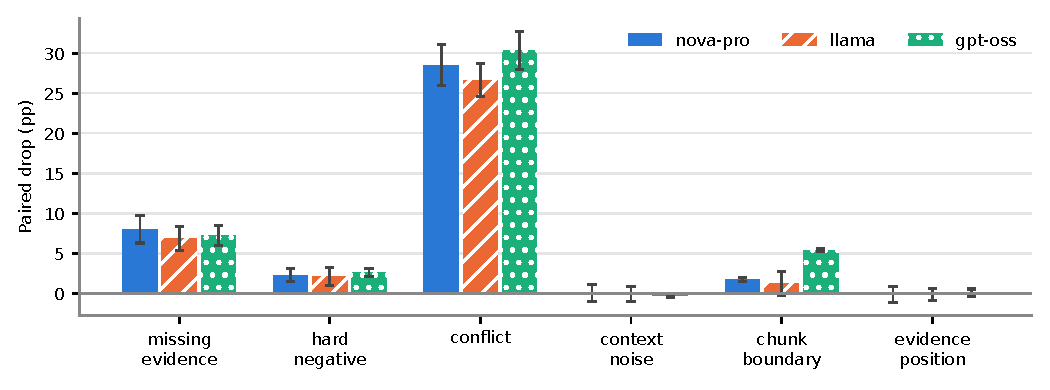
\includegraphics[width=\columnwidth]{figures/fig2_paired_drop.pdf}
\caption{Paired drop by operator, mean over three runs ($\pm$ std). For abstain-expected
operators the drop is the rate of failing to abstain. Every case has eight passages.}
\label{fig:drop}
\end{figure}

Five findings follow (Fig.~\ref{fig:drop}, Tables~\ref{tab:main}--\ref{tab:conflict}).
\emph{First}, the absence operators work: models abstain on 92--93\% of
\op{missing_evidence} and 97--98\% of \op{hard_negative} cases, with 6--7\% and 2\%
hallucinated. Failing to abstain rises with how close the remaining context is to the removed
evidence: 0.0, 7.8 and 15.7 points at low, medium and high severity.
\emph{Second}, \op{conflict} is the dominant failure for every model (26.6--30.4 points, rising
from 12.2 to 28.9 to 44.4 with severity); the three CIs overlap, so it exposes a shared weakness
rather than a ranking, and in 18--26\% of cases the model silently adopts the planted value.
\emph{Third}, \op{context_noise} and \op{evidence_position} cause no drop with eight passages
(every CI includes zero), while \op{chunk_boundary} grows with severity (0.4, 3.0, 5.8) and
separates the models: gpt-oss loses 5.4 points, 3.8--4.6 more than the others
($p_\text{Holm} \le 4\times10^{-7}$). On conflict, gpt-oss differs significantly only from
llama ($-$4.1 points, $p_\text{Holm}$\,=\,0.015).
\emph{Fourth}, how a model fails conflict is model-specific (Table~\ref{tab:conflict}): llama
names both values in 35\% of cases, which a single-answer judge marks wrong, so llama is last on
judge-only accuracy but first on the handled rate. \emph{Fifth}, behavior depends on the prompt
and prior knowledge: allowing the model to flag a conflict raises acknowledgement from 11--35\%
to 59--85\% and the handled rate to 0.89--0.96, and seeds a model answers closed-book are
handled 11--23 points more often than seeds it cannot.

\begin{table}[t]
\centering
\caption{Conflict outcomes (\%), default prompt unless noted, mean over three runs. Handled = gold, both, or acknowledged.}
\label{tab:conflict}
\footnotesize
\setlength{\tabcolsep}{2.4pt}
\resizebox{\columnwidth}{!}{%
\begin{tabular}{@{}lccc@{}}
\toprule
 & nova-pro & llama & gpt-oss \\
\midrule
Gold / alternate / both & 59.3 / 25.8 / 10.4 & 36.8 / 18.2 / 34.9 & 50.4 / 25.2 / 17.5 \\
Acknowledged & 10.6 & 35.1 & 17.6 \\
Handled (judge-only) & 69.7 (69.2) & 72.0 (62.1) & 67.9 (64.2) \\
Handled, prior known / unknown & 86.5 / 63.2 & 78.0 / 66.6 & 78.2 / 58.1 \\
Aware prompt: ack.\ / handled & 58.5 / 88.6 & 83.9 / 95.5 & 84.9 / 95.6 \\
\bottomrule
\end{tabular}}
\end{table}

\subsection{Regression loop on two snapshots}
\label{sec:regression}
Snapshot B re-fetches the same pages on 2026-10-28. In three months 580 of 768 pages have a new
revision and 4 no longer resolve; 11,296 of A's 12,366 chunks are unchanged and B has 13,599.
Of A's 600 seeds, 4.0--6.5\% no longer hold on B (an edited supporting sentence or a changed
answer), about 1.3--2.2\% per month. Rebuilding the benchmark from B with the unchanged
configuration takes 18 minutes and about 4.9k LLM calls; re-fetching the pages takes 188\,s at 8
requests/s and chunking 16\,s. The 3-model evaluation (3.3\,h at a concurrency of 10) dominates
the cost, which scales with models\,$\times$\,cases rather than corpus size. B yields 769
accepted candidates and 188 seeds after the multi-part filter; only 18 of its 200 selected
questions coincide with A's.

The gate compares a candidate run with a baseline per model\,$\times$\,condition and reports
FAIL when the score drops by more than 5 points with a 95\% bootstrap CI below zero (paired when
the benchmark is shared, unpaired when regenerated).
\emph{Knowledge update} (A$\to$B, same system): all 21 cells pass (largest drop 1.5 points, all
CIs include zero; FRS 0.935/0.945/0.924 on A, 0.938/0.955/0.928 on B). Decision: ship.
\emph{Degraded retrieval depth} (B, top-$k$ 8$\to$4, paired): clean accuracy is unchanged
(+0.0 to +1.6 points), so a clean-only test would ship the change. The operators block it in 12
of 21 cells: \op{evidence_position} drops 65--66 points, \op{context_noise} 46--47,
\op{conflict} 8--14 and \op{chunk_boundary} 8--10, all with CIs below zero, because these
operators place the gold passage across all eight slots. FRS falls to 0.71--0.72;
abstain-expected operators are unaffected. Decision: block. The two operators that show no
effect on a correctly configured reader are the ones that catch this configuration error.

\section{Discussion}
\subsection{What a regression points to}
Table~\ref{tab:implications} maps each operator to what it measures and what a regression would
motivate a team to inspect. Because the benchmark presents fixed contexts, it measures the
reader's behavior under each symptom, not the component that would produce the symptom in
production. \op{missing_evidence}, for example, tests whether the generator abstains when
supporting evidence is unavailable; in a production pipeline a similar symptom may motivate
inspecting retrieval coverage, but the benchmark does not measure retriever recall.

\begin{table}[t]
\centering
\caption{What each operator measures, and what a regression may motivate inspecting in a production pipeline (not measured here).}
\label{tab:implications}
\footnotesize
\scriptsize
\begin{tabular}{@{}>{\raggedright\arraybackslash}p{0.25\columnwidth}>{\raggedright\arraybackslash}p{0.38\columnwidth}>{\raggedright\arraybackslash}p{0.3\columnwidth}@{}}
\toprule
Operator & Measured here & May motivate inspecting \\
\midrule
\op{missing_evidence} & Abstention when evidence is absent (92--93\%; 16-point failure at high severity) & Retrieval coverage, indexing \\
\op{hard_negative} & Abstention under near-miss passages (97--98\%) & Retrieval precision, reranking \\
\op{conflict} & Handling of a contradicting copy (27--30-point drop) & Document lifecycle; answer-format prompt \\
\op{chunk_boundary} & Recombining a split sentence (1.2--5.4) & Chunk size, overlap \\
\op{context_noise},\newline \op{evidence_position} & No drop at 8 passages; 46--66 points at top-4 & Retrieval depth, context assembly \\
\bottomrule
\end{tabular}
\end{table}

\subsection{Conflict}
Gold evidence remains present, in full, next to a passage identical except for the answer, and
all three models still lose 27--30 points, adopting the planted value in a fifth to a quarter of
cases. The aware-prompt probe shows the models can detect the contradiction, but the usual
``shortest exact answer'' instruction suppresses it; the closed-book split shows part of the
default-prompt accuracy is parametric recall. A stale but not-yet-purged document is therefore
not something the reader can be relied on to adjudicate.

\subsection{Limitations}
The reader receives fixed contexts; no retriever or reranker is evaluated. The corpus is
English, single-hop Wikipedia; the source adapter is designed for other stores (e.g.\ wikis or
document repositories), but no enterprise connector is evaluated, and scaling claims rest on one
768-page corpus and the throughput measured in Section~\ref{sec:regression}. The human audit
covers 50 seeds and 54 failure cases, and the second annotator was not blind to the first.
Severity levels are configured, not human-validated; 11\% of medium \op{missing_evidence} cases
keep no same-page passage. Context noise and evidence position may stress weaker models or
longer contexts; we did not test them. The multi-part rule was applied to finished runs rather
than at generation time, which leaves 184--189 seeds per run. Clean accuracy is near ceiling by
design, which makes drops attributable to operators but leaves little room to separate
difficulty tiers.

\section{Conclusion}
RAGFailBench regenerates a failure-aware RAG benchmark whenever the corpus changes: validated,
provenance-preserving seeds, a sampled human audit, six typed operators under a fixed context
budget, and a per-operator regression gate. On a Wikipedia pilot it yields a stable funnel
(74.8\% acceptance), an audited seed quality of 84\%, and a clear finding that conflicting
evidence is the dominant failure for three current models. On two real snapshots it ships a
corpus update and blocks a retrieval-depth change that clean accuracy cannot see. Code,
configurations, all runs and the audit sheets are at
\url{https://github.com/taixingbi/RAGFailBench}.

\begin{thebibliography}{99}
\bibitem{lewis2020rag} P. Lewis, E. Perez, A. Piktus, F. Petroni, V. Karpukhin, N. Goyal, H. K\"uttler, M. Lewis, W. Yih, T. Rockt\"aschel, S. Riedel, and D. Kiela, ``Retrieval-augmented generation for knowledge-intensive NLP tasks,'' in \emph{Proc. NeurIPS}, 2020.
\bibitem{gao2023survey} Y. Gao, Y. Xiong, X. Gao, K. Jia, J. Pan, Y. Bi, Y. Dai, J. Sun, and H. Wang, ``Retrieval-augmented generation for large language models: A survey,'' arXiv:2312.10997, 2024.
\bibitem{zhao2024survey} P. Zhao, H. Zhang, Q. Yu, Z. Wang, Y. Geng, F. Fu, L. Yang, W. Zhang, and B. Cui, ``Retrieval-augmented generation for AI-generated content: A survey,'' arXiv:2402.19473, 2024.
\bibitem{huang2024survey} Y. Huang and J. Huang, ``A survey on retrieval-augmented text generation for large language models,'' arXiv:2404.10981, 2024.
\bibitem{ram2023incontext} O. Ram, Y. Levine, I. Dalmedigos, D. Muhlgay, A. Shashua, K. Leyton-Brown, and Y. Shoham, ``In-context retrieval-augmented language models,'' \emph{Trans. Assoc. Comput. Linguist.}, 2023.
\bibitem{es2024ragas} S. Es, J. James, L. Espinosa-Anke, and S. Schockaert, ``RAGAS: Automated evaluation of retrieval augmented generation,'' in \emph{Proc. EACL (System Demonstrations)}, 2024.
\bibitem{saadfalcon2024ares} J. Saad-Falcon, O. Khattab, C. Potts, and M. Zaharia, ``ARES: An automated evaluation framework for retrieval-augmented generation systems,'' in \emph{Proc. NAACL}, 2024.
\bibitem{chen2024rgb} J. Chen, H. Lin, X. Han, and L. Sun, ``Benchmarking large language models in retrieval-augmented generation,'' in \emph{Proc. AAAI}, 2024.
\bibitem{friel2024ragbench} R. Friel, M. Belyi, and A. Sanyal, ``RAGBench: Explainable benchmark for retrieval-augmented generation systems,'' arXiv:2407.11005, 2024.
\bibitem{lyu2024crud} Y. Lyu, Z. Li, S. Niu, F. Xiong, B. Tang, \emph{et al.}, ``CRUD-RAG: A comprehensive Chinese benchmark for retrieval-augmented generation of large language models,'' arXiv:2401.17043, 2024.
\bibitem{shashidhar2025yourbench} S. Shashidhar, C. Fourrier, A. Lozovskaya, T. Wolf, G. Tur, and D. Hakkani-T\"ur, ``YourBench: Easy custom evaluation sets for everyone,'' arXiv:2504.01833, 2025.
\bibitem{liu2024lost} N. F. Liu, K. Lin, J. Hewitt, A. Paranjape, M. Bevilacqua, F. Petroni, and P. Liang, ``Lost in the middle: How language models use long contexts,'' \emph{Trans. Assoc. Comput. Linguist.}, vol. 12, 2024.
\bibitem{cuconasu2024noise} F. Cuconasu, G. Trappolini, F. Siciliano, S. Filice, C. Campagnano, Y. Maarek, N. Tonellotto, and F. Silvestri, ``The power of noise: Redefining retrieval for RAG systems,'' in \emph{Proc. SIGIR}, 2024.
\bibitem{longpre2021entity} S. Longpre, K. Perisetla, A. Chen, N. Ramesh, C. DuBois, and S. Singh, ``Entity-based knowledge conflicts in question answering,'' in \emph{Proc. EMNLP}, 2021.
\bibitem{wu2024clasheval} K. Wu, E. Wu, and J. Zou, ``ClashEval: Quantifying the tug-of-war between an LLM's internal prior and external evidence,'' arXiv:2404.10198, 2024.
\bibitem{rajpurkar2016squad} P. Rajpurkar, J. Zhang, K. Lopyrev, and P. Liang, ``SQuAD: 100,000+ questions for machine comprehension of text,'' in \emph{Proc. EMNLP}, 2016.
\bibitem{kwiatkowski2019nq} T. Kwiatkowski \emph{et al.}, ``Natural Questions: A benchmark for question answering research,'' \emph{Trans. Assoc. Comput. Linguist.}, vol. 7, pp. 453--466, 2019.
\bibitem{joshi2017triviaqa} M. Joshi, E. Choi, D. S. Weld, and L. Zettlemoyer, ``TriviaQA: A large scale distantly supervised challenge dataset for reading comprehension,'' in \emph{Proc. ACL}, 2017.
\bibitem{yang2018hotpotqa} Z. Yang, P. Qi, S. Zhang, Y. Bengio, W. Cohen, R. Salakhutdinov, and C. D. Manning, ``HotpotQA: A dataset for diverse, explainable multi-hop question answering,'' in \emph{Proc. EMNLP}, 2018.
\bibitem{petroni2021kilt} F. Petroni \emph{et al.}, ``KILT: A benchmark for knowledge intensive language tasks,'' in \emph{Proc. NAACL}, 2021.
\bibitem{robertson2009bm25} S. Robertson and H. Zaragoza, ``The probabilistic relevance framework: BM25 and beyond,'' \emph{Found. Trends Inf. Retr.}, vol. 3, no. 4, pp. 333--389, 2009.
\bibitem{karpukhin2020dpr} V. Karpukhin, B. O\u{g}uz, S. Min, P. Lewis, L. Wu, S. Edunov, D. Chen, and W. Yih, ``Dense passage retrieval for open-domain question answering,'' in \emph{Proc. EMNLP}, 2020.
\bibitem{izacard2022contriever} G. Izacard, M. Caron, L. Hosseini, S. Riedel, P. Bojanowski, A. Joulin, and E. Grave, ``Unsupervised dense information retrieval with contrastive learning,'' \emph{Trans. Mach. Learn. Res.}, 2022.
\bibitem{khattab2020colbert} O. Khattab and M. Zaharia, ``ColBERT: Efficient and effective passage search via contextualized late interaction over BERT,'' in \emph{Proc. SIGIR}, 2020.
\bibitem{santhanam2022colbertv2} K. Santhanam, O. Khattab, J. Saad-Falcon, C. Potts, and M. Zaharia, ``ColBERTv2: Effective and efficient retrieval via lightweight late interaction,'' in \emph{Proc. NAACL}, 2022.
\bibitem{thakur2021beir} N. Thakur, N. Reimers, A. R\"uckl\'e, A. Srivastava, and I. Gurevych, ``BEIR: A heterogeneous benchmark for zero-shot evaluation of information retrieval models,'' in \emph{Proc. NeurIPS Datasets and Benchmarks Track}, 2021.
\bibitem{liu2023geval} Y. Liu, D. Iter, Y. Xu, S. Wang, R. Xu, and C. Zhu, ``G-Eval: NLG evaluation using GPT-4 with better human alignment,'' in \emph{Proc. EMNLP}, 2023.
\bibitem{langsmith} LangChain, Inc., ``LangSmith: Evaluation and observability platform for LLM applications,'' docs.smith.langchain.com, 2024.
\bibitem{openaievals} OpenAI, ``Evals: A framework for evaluating LLMs and LLM systems,'' github.com/openai/evals, 2023.
\bibitem{deepeval} Confident AI, ``DeepEval: The open-source LLM evaluation framework,'' github.com/confident-ai/deepeval, 2024.
\bibitem{promptfoo} Promptfoo, ``Open-source LLM testing and evaluation tool,'' github.com/promptfoo/promptfoo, 2024.
\bibitem{liang2022helm} P. Liang, R. Bommasani, T. Lee, D. Tsipras, D. Soylu, M. Yasunaga, \emph{et al.}, ``Holistic evaluation of language models,'' arXiv:2211.09110, 2022.
\bibitem{muennighoff2023mteb} N. Muennighoff, N. Tazi, L. Magne, and N. Reimers, ``MTEB: Massive text embedding benchmark,'' in \emph{Proc. EACL}, 2023.
\bibitem{fowler2006ci} M. Fowler, ``Continuous integration,'' martinfowler.com, 2006.
\bibitem{rothermel1996regression} G. Rothermel and M. J. Harrold, ``Analyzing regression test selection techniques,'' \emph{IEEE Trans. Softw. Eng.}, vol. 22, no. 8, pp. 529--551, 1996.
\bibitem{efron1993bootstrap} B. Efron and R. J. Tibshirani, \emph{An Introduction to the Bootstrap}. Chapman \& Hall, 1993.
\bibitem{mcnemar1947} Q. McNemar, ``Note on the sampling error of the difference between correlated proportions or percentages,'' \emph{Psychometrika}, vol. 12, no. 2, pp. 153--157, 1947.
\bibitem{holm1979} S. Holm, ``A simple sequentially rejective multiple test procedure,'' \emph{Scand. J. Statist.}, vol. 6, no. 2, pp. 65--70, 1979.
\bibitem{cohen1960} J. Cohen, ``A coefficient of agreement for nominal scales,'' \emph{Educ. Psychol. Meas.}, vol. 20, no. 1, pp. 37--46, 1960.
\bibitem{wikipedia} Wikimedia Foundation, ``Wikipedia: The free encyclopedia,'' https://www.wikipedia.org.
\bibitem{mediawiki} Wikimedia Foundation, ``MediaWiki API documentation,'' https://www.mediawiki.org/wiki/API:Main\_page.
\end{thebibliography}

\end{document}
